%======================================================================
\chapter[Evaluation]{Evaluation\footnote{The contents of this 
		chapter have been incorporated within a paper that has been submitted for publication. Qian Liang and Patrick Lam, “MockDetector: Detecting and tracking mock objects in unit tests”. Submitted to 21st IEEE International Working Conference on Source Code Analysis and Manipulation. Submission date June. 30, 2021}}
\label{chap:evaluation}	
%====================================================================== 

We have evaluated \textsc{MockDetector} on 8 open-source benchmarks, along with a micro-benchmark that we developed to test our tool. We ran all of our experiments on a 32-core Intel(R) Xeon(R) CPU E5-4620 v2 at 2.60GHz with 128GB of RAM running Ubuntu 16.04.7 LTS.

Table~\ref{tab:runtimes} presents summary information about our benchmarks and runtimes, namely the LOC and Soot and Doop analysis runtimes for each benchmark. The 9 benchmarks include over 383 kLOC, with 184 kLOC in the test suites, as measured by SLOCCount. The Soot total time is the amount of time that it takes for Soot to analyze the benchmark and test suite in whole-program mode, including our analyses. The Soot intra-procedural analysis time is the sum of runtimes for the main analysis plus two pre-analyses, as described in Section~\ref{sec:soot}. Meanwhile, the reported Doop runtime is from the context-insensitive analysis, while the Doop analysis time for intra-procedural mock invocation analysis is for running the analysis alone based on recorded facts from the benchmark. The total Doop runtime is much slower than the total Soot runtime because Doop always computes a callgraph, which is an expensive operation. We believe that the Doop analysis-only time is also slower because it computes a solution over the entire program, as opposed to Soot, which works one method at a time.
%The major difference between the Doop's total runtime and the actual time spent on mock invocation analysis comes from the build of the complete graph. %Add reference for SLOCCount.

We next investigated the prevalence of mocks. Table~\ref{tab:mocks} presents the number of test-related (Test/Before/After) methods which contain local variables or which access fields that are mocks, mock-containing arrays, or mock-containing collections, as reported by our Soot-based intra-procedural analysis. Across the 8 benchmarks, test-related methods containing local/field mocks or mock-containing containers accounted for 0.35\% to 51.8\% of the total number of test-related methods found in public concrete test classes. Our benchmarks are from different domains and created by different groups of developers. The difference in mock usage reflects their different philosophies and constraints regarding the creation and usage of mock objects in tests. Benchmarks like \textsc{vraptor-core} and \textsc{jsonschema2pojo-core} have more than half of their test-related methods containing mock objects (and mock-containing arrays); in both of these, most field mocks are created via annotations and reused in multiple test cases in the same class.

The core result is in Table~\ref{tab:invokes}, which presents the number of method invocations on mocks detected by our implementations. We present numbers from the imperative intraprocedural Soot implementation, as well as a total of eight versions of the declarative Doop implementation\footnote{bootique, mybatis and vraptor timed out for Doop's 1-object-sensitive analysis without our mock analysis, and we report N/A for their times.}: \{ ``basic-only'' (class hierarchy analysis), ``context-insensitive'' (CI), ``context-insensitive-plusplus'' (CIPP), ``1-object-sensitive'' \} Doop base analysis $\times$ \{ intraprocedural, interprocedural \}. Note that our declarative and imperative implementations find exactly the same number of intraprocedural mock invocations for 4 of our benchmarks. On the others, the main source of missed mock calls in the Soot implementation is from missing support for array or collection related functions. Our intra-procedural analysis finds that method invocations on mock objects account for a range from 0.086\% to 16.4\% of the total number of invocations. 

%--- discuss the numbers for the interprocedural analysis.

In Section~\ref{sec:common} we discussed the implementation of our intraprocedural and interprocedural analyses. We can now discuss the effects of these implementation choices on the experimental results. Recall that we chose, unsoundly, to not propagate any information across method calls in the intraprocedural analysis. Thus, the intraproc columns in Table~\ref{tab:invokes} show smaller numbers than the interproc columns, as expected. The minor difference in \textsc{vraptor-core} is due to one method (which ought to be present) not showing up in Doop's context-insensitive callgraph. Note also that there is a sometimes drastic increase from the intraprocedural to the interprocedural result, e.g. from 40 to 1300 for \textsc{flink}. This is because mocks can (especially context-insensitively) propagate from tests to the methods that they call and all around the main program code. It would be desirable to be able to differentiate test helper methods, which we do want to propagate mocks to, from methods in the main program, which we generally do not want to propagate mocks to; however, our current analysis infrastructure treats test and main code identically.

%We have successfully executed our Doop analysis with different base analyses. We chose to report numbers for the context-insensitive base analysis here as it matches our own analysis. (It would also be possible, but require significantly more effort, to adapt our analysis to carry around context.)

%--- , indicates the removal of mock invocations from call graph would improve the call graph's accuracy on method coverage for the benchmarks on the high end of the mock invocation percentage. 

We explored the run-time performance of our 8 declarative analysis variants based on recorded program facts. We used hyperfine\footnote{https://github.com/sharkdp/hyperfine} to perform 10 benchmarking runs for the souffle command of mock analysis, and present the means and standard deviations from the 10 runs in Table~\ref{tab:doop-intra-runtimes} and~\ref{tab:doop-inter-runtimes}.

The running times show that the Doop runs with basic-only base analysis spend more time on mock analysis for most benchmarks than the runtimes from the more advanced base analyses. Basic-only is a naive base analysis that would generate a much larger call graph than more advanced base analyses, and as it would need to check through more call graph edges, we expect that basic-only would generally spend more time on performing mock analysis. Table~\ref{tab:doop-callgraph-all-counts} highlights the number of source classes and target classes presented in the call graph generated by the four base analyses, which supports the idea that basic-only generates a bigger call graph, and spends most of the extra time checking over unnecessary classes generated in the call graph instead of performing actual mock analysis.

To further investigate on the interprocedural running times on benchmarks include jsonschema2pojo, mybatis, and vraptor, we remove call graph edges that have library classes or dependency classes as source classes for each base analyses, and then count the total number of source classes and target classes in the filtered call graph. As you may see from Table~\ref{tab:doop-callgraph-all-counts}, by taking the difference of the number of target classes from the number of source classes for each base analysis, the numbers suggest that the more advanced base analyses (CI, CIPP) have reached more target classes from a better defined subset of source classes strictly in the benchmark. 

Figure~\ref{fig:edgesToSiblingMethod} shows the call graph edges from method \texttt{<boolean isApplicableType(com.sun.codemodel.JFieldVar)>} to \texttt{java.lang.String fullName()}, which the target method is a sibling method that is first declared in the abstract parent class \texttt{com.sun.codemodel.JType}. From Figure~\ref{fig:edgesToSiblingMethod}, we can tell that basic-only base analyses only report edges to the (abstract) method \texttt{com.sun.codemodel.JType.fullName}, whereas the CHA generated by context-insensitive base analyses would report edges with implementation sites of the target method. Clearly there would be a loss of code coverage from basic-only since it stops at the abstract level. Combining this information with the total number of interprocedural mock invocations reported for the three benchmarks, we know that CI and CIPP have found notably more mock invocations in the process of searching through the edges to the implementation sites of the sibling methods, and the time spent on such process possibly accounts for the higher mock-analysis running times of CI and CIPP on benchmarks jsonschema2pojo, mybatis, and vraptor.


% will discussion more about the call graph edges generated by basic-only in discussion chapter 


\begin{figure}
	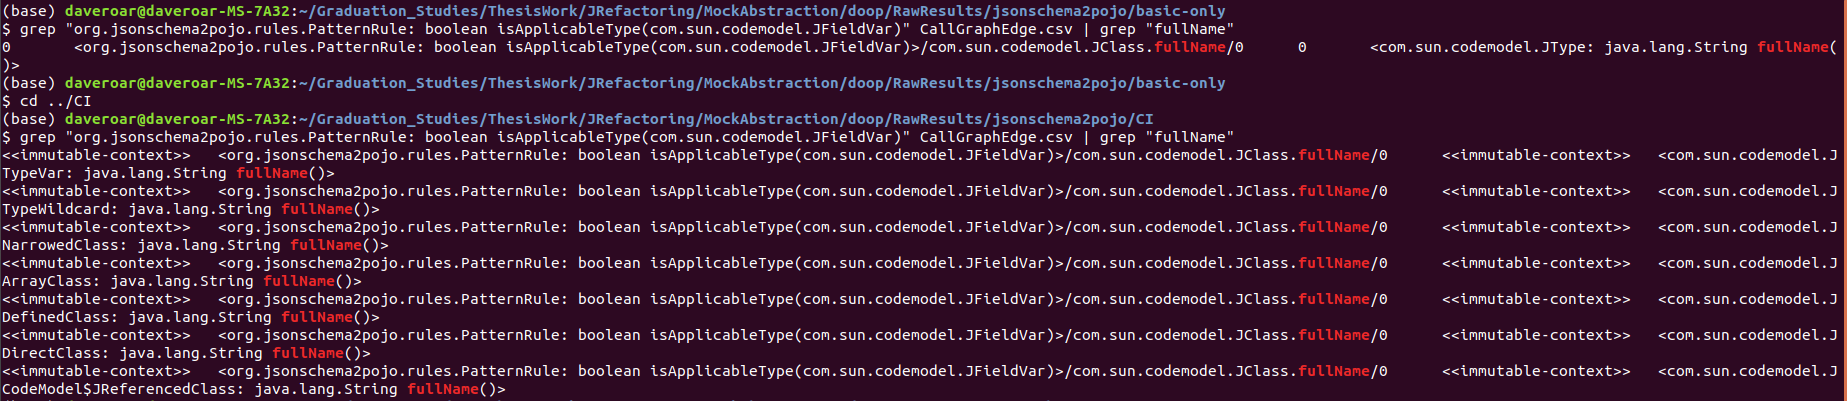
\includegraphics[width=\textwidth,scale=0.8]{Images/EdgesToSiblingMethods.png}
	
	\caption{The call graph edges to a sibling method \textit{fullName()} from .}
	\label{fig:edgesToSiblingMethod}
	
\end{figure}
% More discussion will be added for the outlier: mybatis and vraptor interprocedural runtimes.

In addition, we can observe that CI and CIPP have comparable runtimes and mock invocation counts, with CI has slightly higher runtimes, both intra-procedurally and inter-procedurally. It makes sense as CIPP is "context-insensitive with an enhancement for low-hanging fruit: methods that have their params flow to their return value get a methods that have their params flow to their return value get a 1-obj treatment"~\cite{yanniss}. Data presented in Table~\ref{tab:doop-callgraph-all-counts} demonstrates that the call graph sizes are comparable for CI and CIPP, with CI's call graphs generally slightly bigger as expected.

On the other hand, since 1-object-sensitive base analysis is a more sophisticated analysis, it spends much longer time on building the CHA graph (3 benchmarks ending up with timed out runs on building the CHA graph), resulting in a much smaller call graph and thus has a faster execution time on actual mock analysis. 

% We are currently investigating the performance of intra-procedural basic-only analysis, trying to understand why it would spend more time strictly on mock analysis than CI and CIPP.

%the number of mock invocations correlates with the runtime; taking a bit more effort to compute a better call graph may well pay off in terms of overall analysis time. We suspect that the interprocedural analysis is especially slow for mybatis because we also analyze its 50 dependencies; that count is at the high end among our benchmarks.

\begin{table*}
	\centering
	\caption{Our suite of 8 open-source benchmarks (8000--117000 LOC) plus our microbenchmark. Soot and Doop analysis runtimes.}
	%	\begin{adjustbox}{width=0.1\textwidth}
	\vspace*{.5em}
	\resizebox{\columnwidth}{!}{%
	\begin{tabular}{lrrrrrr}
		\toprule
		Benchmark & Total LOC & Test LOC & \thead{Soot intraproc \\ total time (s)} & \thead{Doop intraproc \\ total time (s)} & \thead{Soot intraproc \\ mock analysis (s)}  & \thead{Doop intraproc \\ mock analysis (s)} \\
		\midrule
		bootique-2.0.B1-bootique           		&  15530   & 8595   & 58  & 2810  &  0.293   & 19.93       \\
		commons-collections4-4.4           		&  65273   & 36318  & 114 & 694   &  0.345   & 14.20       \\
		flink-core-1.13.0-rc1           		&  117310  & 49730  & 341 & 1847  &  0.358   & 27.21        \\
		jsonschema2pojo-core-1.1.1         		&  8233    & 2885   & 313 & 1005   &  0.282   & 29.33       \\
		maven-core-3.8.1   		           		&  38866   & 11104  & 183 & 588   &  0.192   & 19.49        \\
		micro-benchmark         		  		&  954     & 883	& 47  & 387   &  0.126   & 11.73        \\
		mybatis-3.5.6         		  			&  68268   & 46334  & 500 & 4477  &  0.524   & 59.83        \\
		quartz-core-2.3.1        	  			&  35355   & 8423   & 155 & 736   &  0.215   & 21.06     \\
		vraptor-core-3.5.5         	  			&  34244   & 20133  & 371 & 1469  &  0.340   & 34.95      \\
		\bottomrule
		Total         	  						&  384033  & 184405 & 2082 & 14013 &  2.675  & 237.73     \\
	\end{tabular}
	}
	%	\end{adjustbox}
	\label{tab:runtimes}
\end{table*}

\begin{table*}
	\centering
	\caption{Counts of Test-Related (Test/Before/After) methods in public concrete test classes, along with counts of mocks, mock-containing arrays, and mock-containing collections, reported by Soot intraprocedural analysis.}
	%	\begin{adjustbox}{width=0.1\textwidth}
	\vspace*{.5em}
	\begin{tabular}{lrrrr}
		\toprule
		Benchmark & \thead{\# of Test-Related \\ Methods} & \thead{\# of Test-Related \\ Methods with \\ mocks (intra)}  & \thead{\# of Test-Related \\ Methods with \\ mock-containing\\ arrays (intra)} & \thead{\# of Test-Related \\ Methods with \\ mock-containing\\ collections (intra)} \\
		\midrule
		bootique-2.0.B1-bootique           		&  420        &  32  & 7 & 0       \\
		commons-collections4-4.4          		&  1152       &  3   & 1 & 1       \\
		flink-core-1.13.0-rc1           		&  1091       &  4   & 0 & 0       \\
		jsonschema2pojo-core-1.1.1           	&  145        &  76  & 1 & 0       \\
		maven-core-3.8.1	           			&  337        &  24  & 0 & 0       \\
		micro-benchmark         		  		&  59         &  43  & 7 & 25       \\
		mybatis-3.5.6         		  			&  1769       &  330 & 3 & 0       \\
		
		quartz-core-2.3.1         	  			&  218     	  &  7   & 0 & 0      \\
		vraptor-core-3.5.5         	  			&  1119       &  565 & 15 & 0      \\
		\bottomrule
		Total        	  						&  6310       &  1084  & 34 & 26    \\
	\end{tabular}
	%	\end{adjustbox}
	\label{tab:mocks}
\end{table*}

\begin{landscape}
\begin{table*}
	\ra{1.2}
	\centering
	\caption{Comparison of Number of InstanceInvokeExprs on Mock objects analyzed by Soot and Doop, and Total Number of InstanceInvokeExprs, in each benchmark's test suite. ``--'' = timed out after 90 minutes.}
	\vspace*{.5em}
	\begin{tabular}{@{}lrrcrrrrcrrrr@{}} \toprule
	Benchmark & \thead{Total \\ Number of \\ Invocations} & \thead{Mock Invokes \\ intraproc (Soot)}
	& \phantom{abc} & \multicolumn{4}{c}{intraproc} & \phantom{abc} & \multicolumn{4}{c}{interproc}
	\\
	\cmidrule{5-8} \cmidrule{10-13}
	& & & & \thead{basic\\-only} & CI & CIPP & \thead{1-obj\\-sens} & & \thead{basic\\-only} & CI & CIPP & \thead{1-obj\\-sens} \\ \midrule
	\csvreader[head to column names, late after line=\\]
	{Data/DoopAndSootMockCounts.csv}{}%
	{\csvcoli&\csvcolii&\csvcoliii&&\csvcoliv&\csvcolv&\csvcolvi&\csvcolvii& &\csvcolviii&\csvcolix&\csvcolx&\csvcolxi}
	\bottomrule
	\end{tabular}
	\label{tab:invokes}
\end{table*} 
\end{landscape}

%\begin{table*}
%	\centering
%	\caption{Comparison of Number of InstanceInvokeExprs on Mock objects analyzed by Soot and Doop, and Total Number of InstanceInvokeExprs, in each benchmark's test suite. N/A = timed out after 90 minutes.}
%	%	\begin{adjustbox}{width=0.1\textwidth}
%	\begin{tabular}{lrrrrrr}
%		\toprule
%		Benchmark & \thead{Total Number \\ of Invocations} & \thead{Mock Invokes \\ intraproc (Soot)} & \thead{Basic-only, \\ intraproc (Doop)} & \thead{Context-insensitive, \\ intraproc (Doop)} &  \thead{Basic-only, \\ interproc (Doop)} &\thead{Context-insensitive, \\ interproc (Doop)} \\
%		\midrule
%		bootique-2.0.B1-bootique           		&  3366     &  99   & 99    & 99   & 120   & 122    \\
%		commons-collections4-4.4       			&  12753    &  11   & 0     &  3   & 0    & 23   \\
%		flink-core-1.13.0-rc1           		&  11923    &  40   & 40    & 40   & 1262  & 1389   \\
%		jsonschema2pojo-core-1.1.1      	     	&  1896     &  276  & 282   & 282  & 462   & 604   \\
%		maven-core-3.8.1           			&  4072     &  23   & 23    & 23   & 31    & 39  \\
%		microbenchmark         		  		&  471      &  108  & 123   & 123  & 132   & 132   \\
%		mybatis-3.5.6         		  		&  19232    &  575  & N/A   & 577  &  N/A  & 1345     \\
%		quartz-core-2.3.1       	  		&  3436     &  21   & 21    & 21   & 23    & 31    \\
%		vraptor-core-3.5.51        	  		&  5868     &  942  & 963   & 962  & 1301  & 1630   \\
%		\bottomrule
%		Total        	  				&  63017    & 2095  & N/A   & 2130  & N/A  & 5315   \\
%	\end{tabular}
%	%	\end{adjustbox}
%	\label{tab:invokes}
%\end{table*}

%& & \thead{basic\\-only} & $\sigma$ & CI & $\sigma$ & CIPP & $\sigma$ & \thead{1-obj\\-sens} & $\sigma$ \\


\begin{table*}
	\centering
	\caption{Intra-procedural Doop analysis-only runtime (in seconds) after basic-only, context-insensitive, context-insensitive-plusplus and 1-object-sensitive base analyses. \protect\\ ``--'' = timed out after 90 minutes.}
	\vspace*{.5em}
	\begin{tabular}{@{}lrrrrrrrr} \toprule
		Benchmark & \multicolumn{8}{c}{intraproc}\\
		\cmidrule{2-9}
		& \thead{basic\\-only} & $\sigma$ & CI & $\sigma$ & CIPP & $\sigma$ & \thead{1-obj\\-sens} & $\sigma$ \\ \midrule 
		
		\csvreader[head to column names, late after line=\\]
		{Data/HyperfineRuntimeWithAvgsINTRA.csv}{}%
		{\csvcoli&\csvcolii&{\scriptsize \csvcoliii}&\csvcoliv&{\scriptsize \csvcolv} &\csvcolvi&{\scriptsize \csvcolvii}&\csvcolviii &{\scriptsize \csvcolix}}
		\bottomrule
	\end{tabular}
	\label{tab:doop-intra-runtimes}
\end{table*}

\begin{table*}
	\centering
	\caption{Inter-procedural Doop analysis-only runtime (in seconds) after basic-only, context-insensitive, context-insensitive-plusplus and 1-object-sensitive base analyses. \protect\\ ``--'' = timed out after 90 minutes.}
	\vspace*{.5em}
	\begin{tabular}{@{}lrrrrrrrr} \toprule
		Benchmark & \multicolumn{8}{c}{interproc}\\
		\cmidrule{2-9}
		& \thead{basic\\-only} & $\sigma$ & CI & $\sigma$ & CIPP & $\sigma$ & \thead{1-obj\\-sens} & $\sigma$ \\ \midrule 
		
		\csvreader[head to column names, late after line=\\]
		{Data/HyperfineRuntimeWithAvgsINTER.csv}{}%
		{\csvcoli&\csvcolii&{\scriptsize \csvcoliii}&\csvcoliv&{\scriptsize \csvcolv} &\csvcolvi&{\scriptsize \csvcolvii}&\csvcolviii &{\scriptsize \csvcolix}}
		\bottomrule
	\end{tabular}
	\label{tab:doop-inter-runtimes}
\end{table*}


\begin{table*}
	\centering
	\caption{Total number of source classes and target classes found in the call graph generated from inter-procedural Doop analysis with basic-only, context-insensitive, context-insensitive-plusplus, and 1-object-sensitive base analyses. ``--'' = timed out after 90 minutes.}
	\vspace*{.5em}
	\begin{tabular}{@{}lrrrrcrrrr} \toprule
		Benchmark & \multicolumn{4}{c}{Source Classes} & \phantom{abc} & \multicolumn{4}{c}{Target Classes}
		\\
		\cmidrule{2-5} \cmidrule{7-10}
		& \thead{basic\\-only} & CI & CIPP & \thead{1-obj\\-sens} & & \thead{basic\\-only} & CI & CIPP & \thead{1-obj\\-sens} \\ \midrule
		\csvreader[head to column names, late after line=\\]
		{Data/CallGraphEdgeClassCounts.csv}{}%
		{\csvcoli&\csvcolii&\csvcoliii&\csvcoliv&\csvcolv&&\csvcolvi&\csvcolvii&\csvcolviii&\csvcolix}
		\bottomrule
	\end{tabular}
	\label{tab:doop-callgraph-all-counts}
\end{table*}

\begin{table*}
	\centering
	\caption{Total number of source classes in the root package of the benchmark (i.e., excluding classes from dependencies or libraries), and target classes reachable from the corresponding source classes found in the call graph generated from inter-procedural Doop analysis with basic-only, context-insensitive, context-insensitive-plusplus, and 1-object-sensitive base analyses. ``--'' = timed out after 90 minutes.}
	\vspace*{.5em}
	\begin{tabular}{@{}lrrrrcrrrr} \toprule
		Benchmark & \multicolumn{4}{c}{Source Classes} & \phantom{abc} & \multicolumn{4}{c}{Target Classes}
		\\
		\cmidrule{2-5} \cmidrule{7-10}
		& \thead{basic\\-only} & CI & CIPP & \thead{1-obj\\-sens} & & \thead{basic\\-only} & CI & CIPP & \thead{1-obj\\-sens} \\ \midrule
		\csvreader[head to column names, late after line=\\]
		{Data/CallGraphEdgePackageClassCounts.csv}{}%
		{\csvcoli&\csvcolii&\csvcoliii&\csvcoliv&\csvcolv&&\csvcolvi&\csvcolvii&\csvcolviii&\csvcolix}
		\bottomrule
	\end{tabular}
	\label{tab:doop-callgraph-package-counts}
\end{table*}

%\begin{table*}
%	\centering
%	\caption{Doop analysis-only runtime after basic-only, context-insensitive, context-insensitive-plusplus and 1-object-sensitive base analyses. N/A = timed out after 90 minutes.}
%	%	\begin{adjustbox}{width=0.1\textwidth}
%	\begin{tabular}{lrrrrrr}
%		\toprule
%		Benchmark & \thead{Basic-only, \\ intraproc (s)} & \thead{Context-insensitive, \\ intraproc (s)} & \thead{Basic-only, \\ interproc (s)}  & \thead{Context-insensitive, \\ interproc (s)}  \\
%		\midrule
%		bootique-2.0.B1-bootique           		& 15.71  & 16.81 &  24.26    &  20.20     \\
%		commons-collections4-4.4           		& 17.42  & 12.26 &  21.79    &  15.36        \\
%		flink-core-1.13.0-rc1           		& 24.67  & 25.30 &  71.67    &  66.10         \\
%		jsonschema2pojo-core-1.1.1         		& 25.98  & 26.27 &  42.14    &  39.21         \\
%		maven-core-3.8.1   		        	& 18.01  & 16.34 &  25.49    &  22.09          \\
%		micro-benchmark         			& 10.97  & 10.50 &  12.51    &  12.53        \\
%		mybatis-3.5.6         		  		&  N/A   & 51.25 &   N/A     & 183.86          \\
%		quartz-core-2.3.1        	  		& 17.72  & 19.83 &  22.99    &  21.14        \\
%		vraptor-core-3.5.5         	  		& 22.10  & 23.81 &  66.73    & 146.09       \\
%		\bottomrule
%	\end{tabular}
%	%	\end{adjustbox}
%	\label{tab:doop-runtimes}
%\end{table*}
